\documentclass[border={1pt 0pt 0pt 0pt}]{standalone}
\usepackage{pgfplots}
\usepackage{tikz}
\usepackage{xcolor}
\usetikzlibrary{calc,patterns,angles,quotes}
\begin{document}

  % \begin{tikzpicture}
  %   \coordinate (origo) at (0,0);
  %   \coordinate (pivot) at (1,5);
  %   % draw axes
  %   \fill[black] (origo) circle (0.05);
  %   \draw[thick,gray,->] (origo) -- ++(4,0) node[black,right] {$x$};
  %   \draw[thick,gray,->] (origo) -- ++(0,-4) node (mary) [black,below] {$y$};
  %   % draw roof
  %   \fill[pattern = north east lines] ($ (origo) + (-1,0) $) rectangle ($ (origo) + (1,0.5) $);
  %   \draw[thick] ($ (origo) + (-1,0) $) -- ($ (origo) + (1,0) $);
  %   \draw[thick] (origo) -- ++(300:3) coordinate (bob);
  %   \fill (bob) circle (0.2);
  %   \pic [draw, ->, "$\theta$", angle eccentricity=1.5] {angle = mary--origo--bob};
  % \end{tikzpicture}

  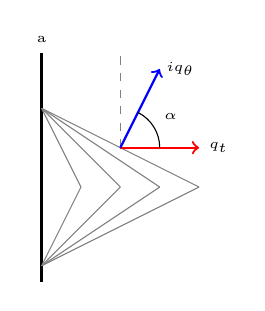
\begin{tikzpicture}
    \coordinate (point) at (1,0.5);
    \draw[thick] (0,1.7) node[above] {{\tiny $\mathrm{a}$}} -- (0,-1.2);
    % \draw[dashed] (point) -- (2.1,2.7);
    % \draw[dashed,gray] (point) -- (2.1,0.5);
    \draw[dashed,gray] (point) -- (1,1.7);
    \foreach \p in {0.5,1,1.5,2}{
      \draw[gray] (0,1) -- (\p,0);
      \draw[gray] (0,-1) -- (\p,0);
      }
    \draw[thick,red,->] (point) -- (2,0.5)
    node (time) [black,right] {{\tiny $q_t$}};
    \draw[thick,blue,->] (point) -- (1.5,1.5)
    node (theta) [black] {\quad \, {\tiny $iq_{\theta}$}};
    \pic [draw, "{\tiny $\alpha$}", angle eccentricity=1.5] {angle = time--point--theta};
  \end{tikzpicture}

\end{document}


